
\chapter{Memory accesses}\label{Accesses}

We will now address a completely different topic and return to our main concern, which is to adapt a data structure to the graphics card. We wanted to start by studying memory behavior. Indeed, this is a crucial element when developing a data structure where we try to minimize the number of steps to find an element as well as the number of cells or cache lines that we must consult to guide our queries. As a matter of fact, the computation model on GPU proposes minimum units of parallelism that group the elements by warp, a same instruction is executed by, generally, 32 threads at the same time and the same goes for the memory access instructions. We can therefore study the variety of accesses that the whole warp can perform at the same time.

\section{Type of accesses}

We wanted to study the behavior of 4 main different types of access. First, how long it took to search for one and only one item. This will allow us to define our base case, and compare it with other accesses, get the minimal running time to issue those actions. Secondly, we wanted to know what the impact was if all the elements of the same warp tried to access the same element. Indeed, Cuda indicates us that the accesses will then be serialized. Third, Cuda recommends accessing coalesced\index{Coalesced} or at least adjacent addresses, so threads will all access contiguous elements in memory but not necessarly coalesced~\cite{harris2007optimizing}. Finally, the question arose for random accesses, if each thread accessed a different and non-contiguous element in memory which would represent the worst scenario among these. The other possible types of access are of less interest to us since they seem to be placed in intermediate positions and not sufficiently relevant.

\begin{figure}[ht] 
  \label{TypeOfAccesses} 
  \begin{minipage}[b]{0.5\linewidth}
    \centering
    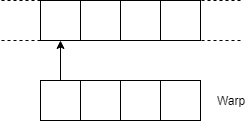
\includegraphics[width=.5\linewidth]{Chapters/Accesses/access-OnlyOne.png} 
    \caption{Only one} 
    \vspace{4ex}
  \end{minipage}%%
  \begin{minipage}[b]{0.5\linewidth}
    \centering
    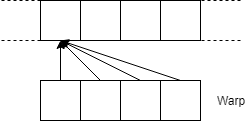
\includegraphics[width=.5\linewidth]{Chapters/Accesses/access-SameOne.png} 
    \caption{Same one} 
    \vspace{4ex}
  \end{minipage} 
  \begin{minipage}[b]{0.5\linewidth}
    \centering
    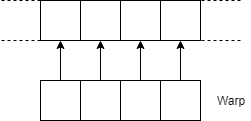
\includegraphics[width=.5\linewidth]{Chapters/Accesses/access-Adjacent.png} 
    \caption{Adjacent} 
    \vspace{4ex}
  \end{minipage}%% 
  \begin{minipage}[b]{0.5\linewidth}
    \centering
    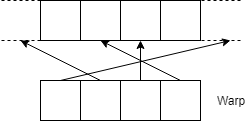
\includegraphics[width=.5\linewidth]{Chapters/Accesses/access-random.png} 
    \caption{Random} 
    \vspace{4ex}
  \end{minipage} 
  \caption{Different pattern of accesses}
\end{figure}

\section{Experiment}

We designed a relatively simple experiment. We start by reserving a large amount of memory, 2GB. Then, each thread accesses its own element according to its defined access policy. 16 million accesses ($2^{24}$) are made in order to saturate the memory and avoid cache phenomena. Those positions are determined by a pseudo-random function (hash function) based on the current step in the algorithm and an initial random offset. A very simple operation is then performed with the loaded element, an incrementation. The experiment is performed on objects of different sizes: 4 bytes, 8 bytes, 16 bytes and 32 bytes in order to see the impact of size evolution on performance.

We performed the experiment in various configurations by varying the number of warps and blocks, in order to obtain the Cartesian product from 1 to 32 ($2^{5}$) for warps and 1 to 1024 ($2^{10}$) for blocks, by doubling steps (matrices of $5 \times 10$). We collected the result of 10 runs, each receives a different original offset for the position, and performed 10 iterations each time, to reduce the cost of launching one kernel. Various statistical elements are then collected, in particular moments or quantiles.

\section{Results}

As the results depend on many factors: the type of access, the size of the data, the number of warps and the number of groups, we present a non-exhaustive view of the results. Please note the scales vary from one result representation to another. We will try to extract the key elements of the experiment and present them and we will quickly move on to elements that we have found less relevant.

\begin{figure}[!ht]
  \begin{minipage}[b]{0.5\linewidth}
    \centering
    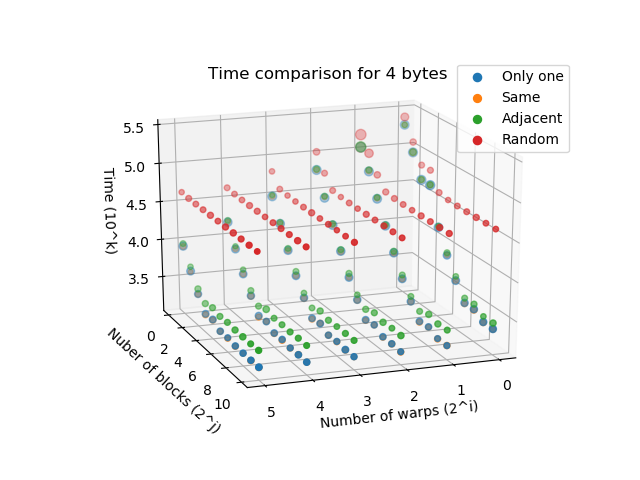
\includegraphics[width=\linewidth]{Chapters/Accesses/4bytesaccesses.png} 
    \caption{Time to access to 4 bytes} 
    \vspace{4ex}
  \end{minipage}%%
  \begin{minipage}[b]{0.5\linewidth}
    \centering
    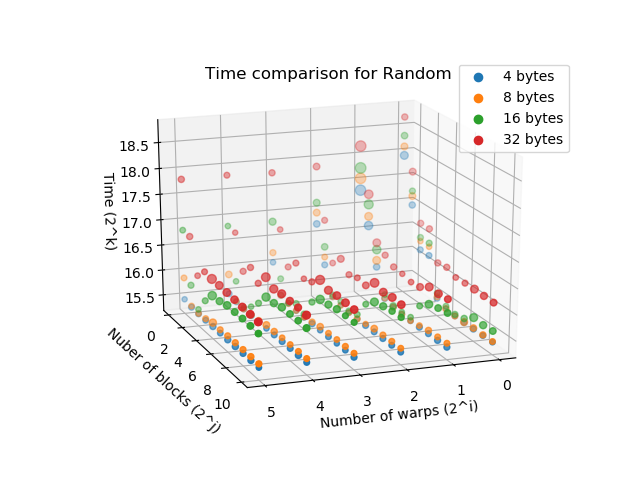
\includegraphics[width=\linewidth]{Chapters/Accesses/Random.png} 
    \caption{Time for random accesses} 
    \vspace{4ex}
  \end{minipage} 
\end{figure}

Several remarks can be made on the first and raw results:
\begin{itemize}
    \item Access times stabilize relatively quickly, and adding new warps or groups does not save time beyond one configuration. This corresponds quite naturally to the saturation of the bandwidth. Indeed, we are not able to issue more accesses than the memory is able to offer in the same time interval.
    \item We achieve the maximal bandwidth possible in all the cases if we consider that the elements are loaded in cache\index{Block} line of 128 bytes. We also remark that the practical bandwidth is lower than the theoretical one (we get about 100GB/s instead of the 112GB/s), this may be due to the inner latency of these instructions (12 cycles for issue latency - time to start the instruction - and 172 for the whole latency - time before being able to start a new instruction - as reported by the gpuperformance tool~\cite{gpuperformance}).
    \item When the random accesses on 16 and 32 bytes exceed a certain configuration (number of warps $\times$ number of blocks $\geq$ constant), the access time increases slightly to stabilize with a higher variance. This may be due to a stronger eviction in the cache\index{Cache} due to the pressure on it which is increasing.\\
\end{itemize}

These raw data are not really surprising by themselves but when we compare the performances between them, we can observe some other aspects where the results are quite surprising:

\begin{figure}[!ht]
  \begin{minipage}[b]{0.5\linewidth}
    \centering
    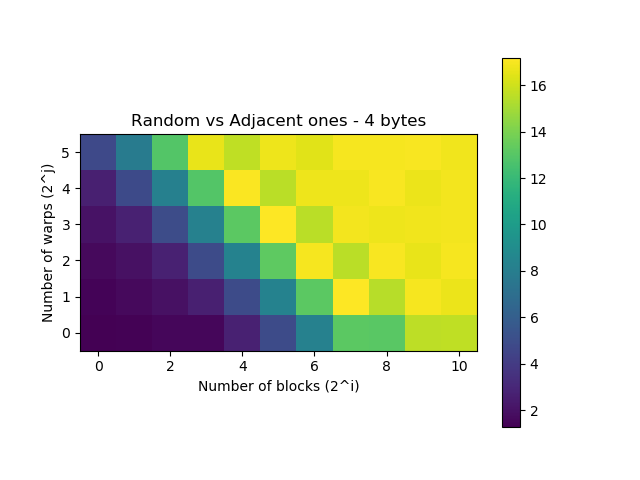
\includegraphics[width=\linewidth]{Chapters/Accesses/RandomvsAdjacentones4bytes.png} 
    \caption{Slowdown between adjacent\\ and random accesses on 4 byte elements} 
    \vspace{4ex}
  \end{minipage}%%
  \begin{minipage}[b]{0.5\linewidth}
    \centering
    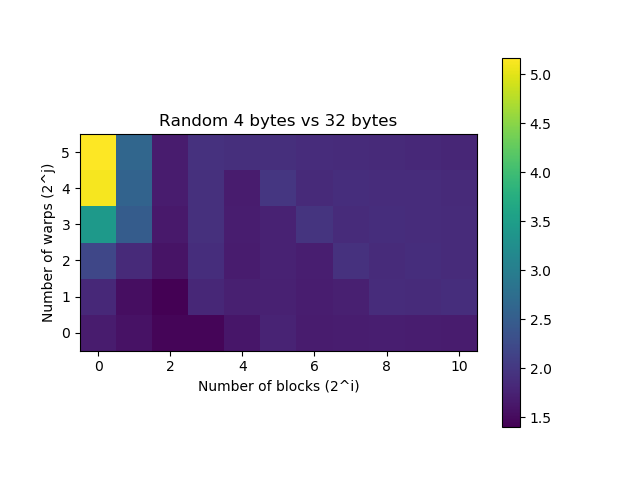
\includegraphics[width=\linewidth]{Chapters/Accesses/Random4bytesvs32bytes.png} 
    \caption{Slowdown between random accesses on 4 bytes and 32 bytes} 
    \label{fig:randomaccesses4vs32}
    \vspace{4ex}
  \end{minipage} 
\end{figure}

Indeed, we would expect to have a slowndown factor of $32$ since the random data are spread randomly in $32$ different cache\index{Block} lines, but we only get $16$. This is due to the fact that the elements are not coalesced\index{Coalesced} and thus we need to load $2$ cache\index{Block} lines in average for adjacent strategy. But if we increase the size of the data, the slowing factor becomes less and less important, with sizes of $8$ and $16$ bytes, we are only at a factor of about $12$ and $8$ respectively and when we go to $32$ bytes (which is quite large), the numbers collapse to $3.5$. It becomes to be more interesting to perform random accesses than the equivalent amount of sequential.

Curiously, we observe that the time to obtain the data is noticably sublinear with the data size and not directly proportional, this would suggest that a mecanism of prefetching is provided by default and, in the case of random accesses, the cost is essentially free since the cache\index{Block} lines are already loaded. The upper left corner of the figure~\ref{fig:randomaccesses4vs32} remains a complete mystery.

From this small experience, we can conclude a very important point. Accessing the data in an adjacent manner is always more interesting but the gap becomes smaller and smaller compared to random if you need a lot of data. This is a direct consequence of a rather logical phenomenon. The bandwidth remains the same no matter what happens, what changes mainly is the efficiency of the data loaded. It is better to consult all the cells obtained during a random access and thus compact the data in this case, whereas the sequential case will be better on average.

In addition, and in the course of this work, we have noticed several times that we have been confronted with memory dependency problems. The mechanism used to hide the latency of instructions was not sufficiently effective and a significant amount of time could be lost on this aspect, which also led to data dependency and execution issues. This was especially the case for hash tables.